\section{Аналитический раздел}
\label{sec:analytics}

\subsection{Статистика потерянных и найденных вещей}

Для подтверждения актуальности и важности разрабатываемой системы, необходимо провести исследование рынка и определить основные проблемы и потребности пользователей. Одним из способов сбора информации является проведение опроса среди пользователей.

Одним из основных факторов, определяющих актуальность разрабатываемой системы является статистика потерянных и найденных вещей. Необходимо определить количество потерянных вещей в месяц, год и за весь период работы системы. Это поможет оценить нагрузку на систему и определить ее производительность.

Статистика, взятая с сайта столнаходок.рф~\cite{bib:stol_nahodok}, утверждает, что только 20~\% пользователей их сайта смогли установить и вернуть вещи. Также на рисунках \ref{fig:chart2023} и \ref{fig:chart2022} представлена гистограмма количества созданных объявлений за 2022 и 2023 года.

\begin{figure}[htb]
	\centering
	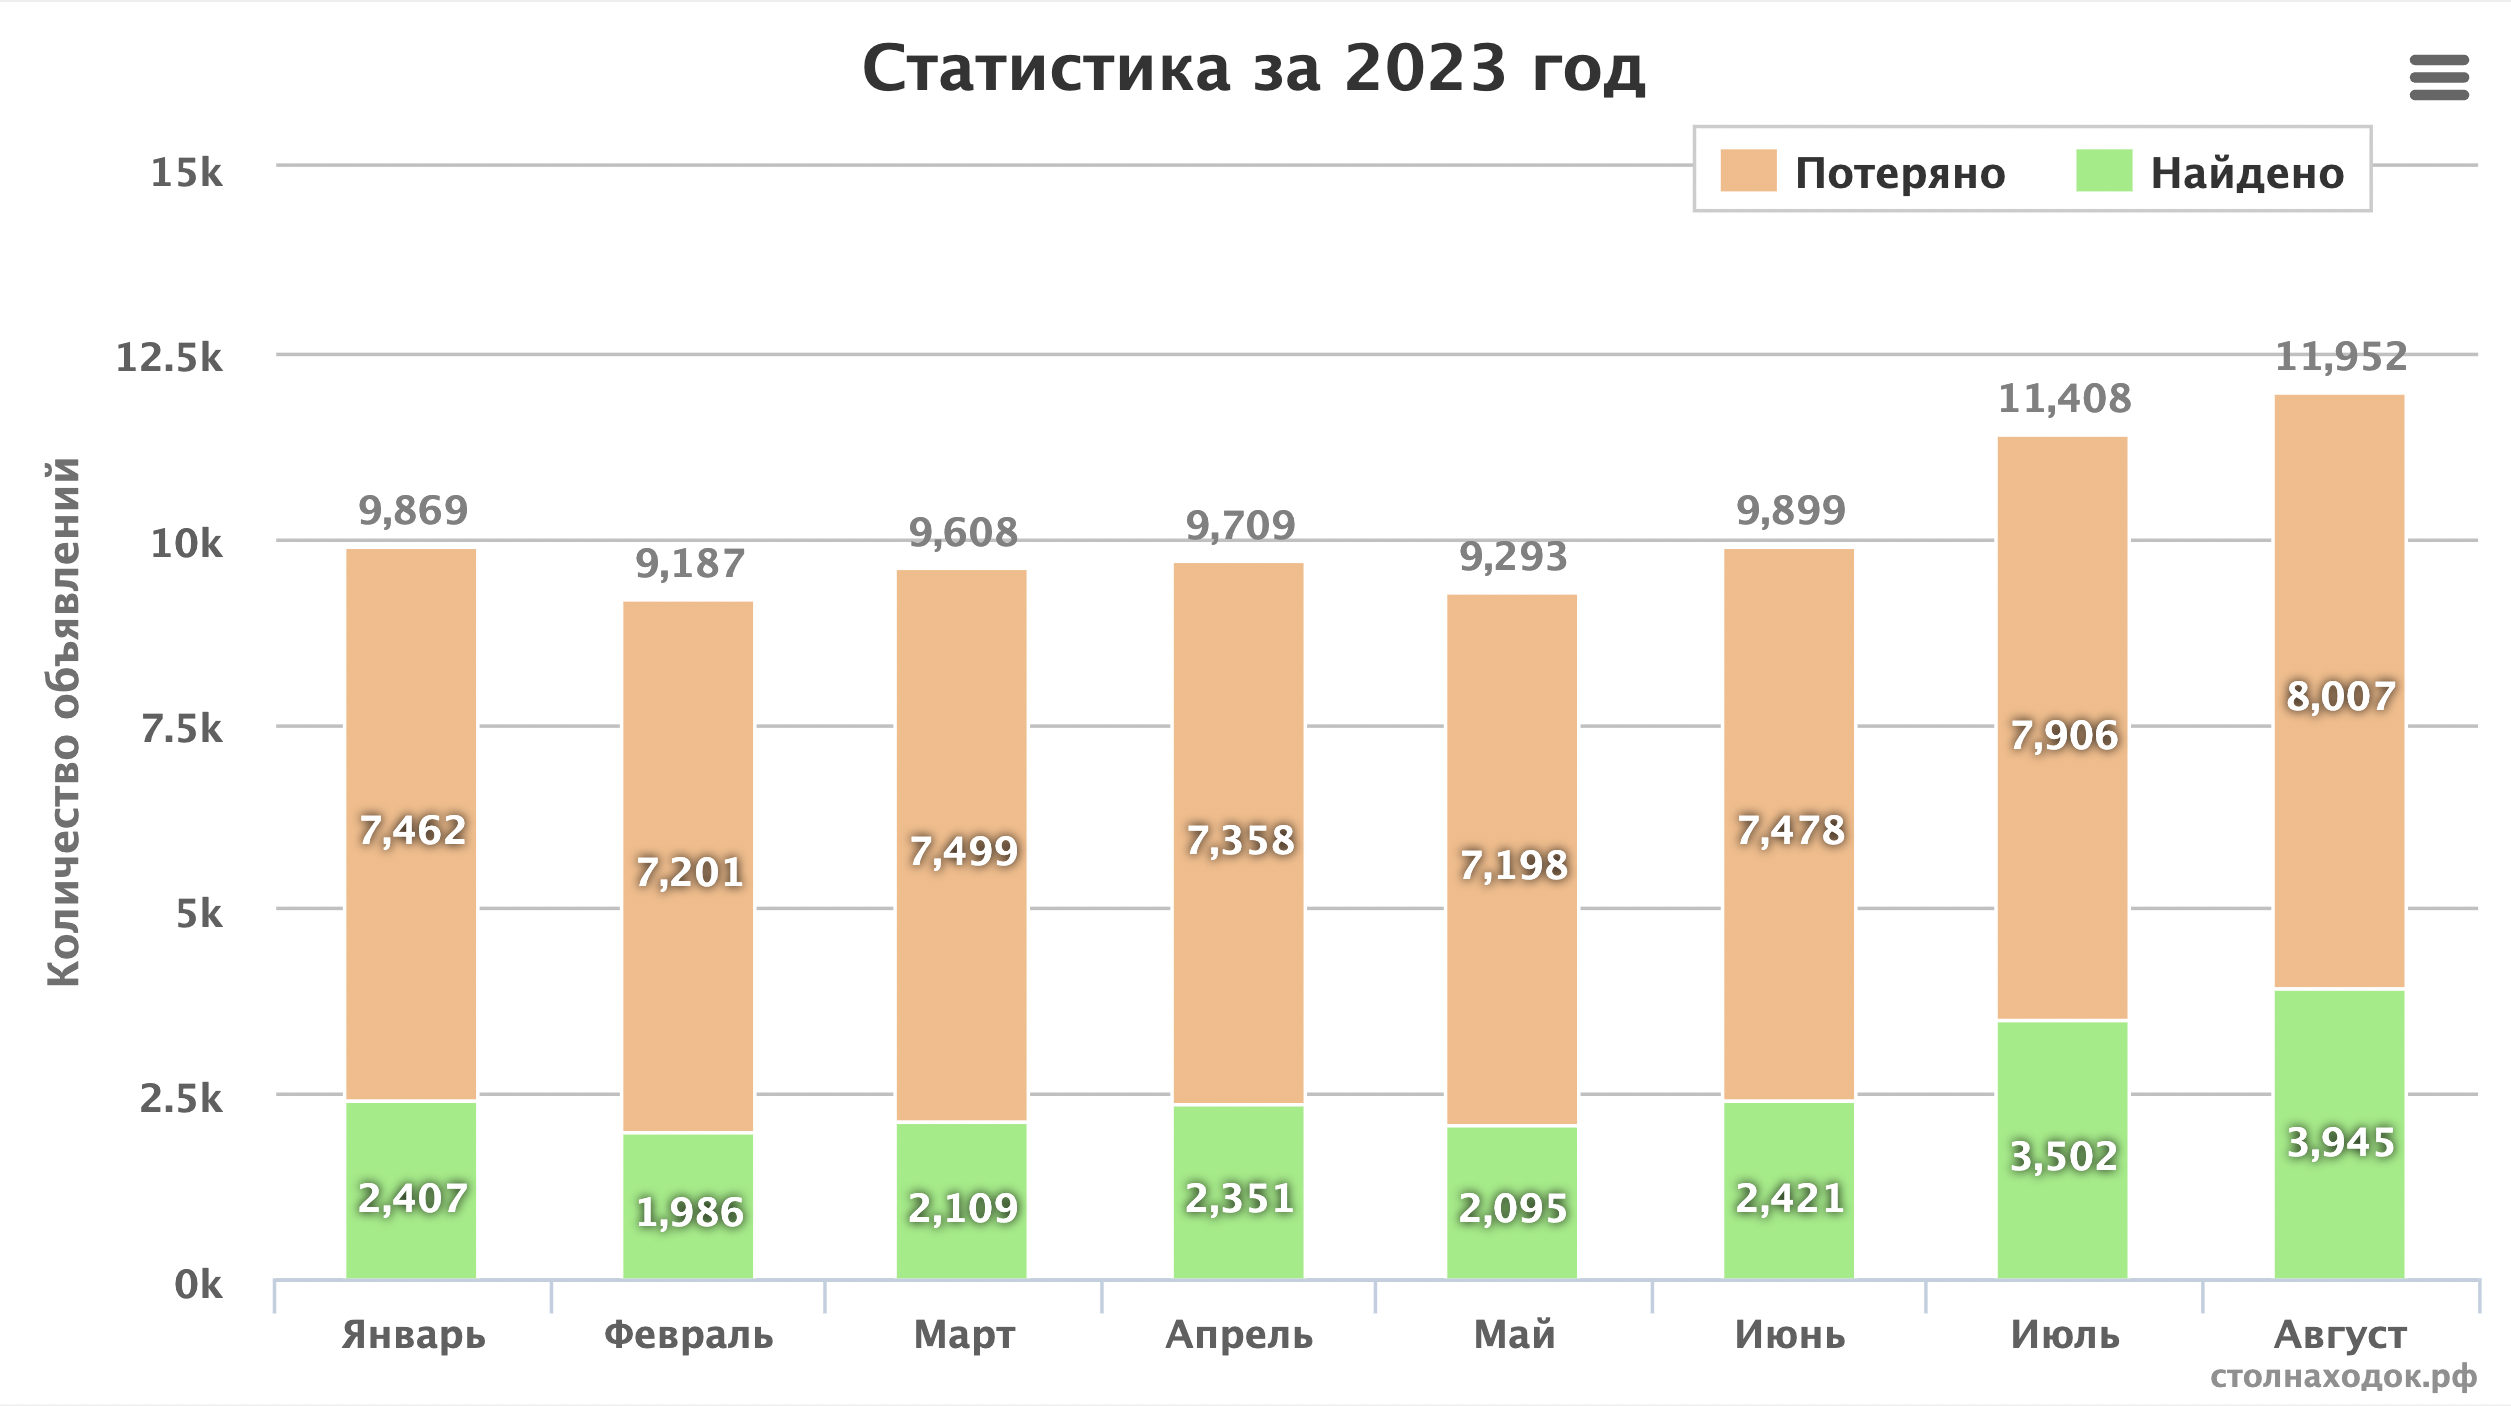
\includegraphics[width=.6\textwidth]{images/chart2023}
	\parskip=6pt
	\caption{Востребованность системы столнаходок.рф в 2023 году}
	\label{fig:chart2023}
\end{figure}

\begin{figure}[htb]
	\centering
	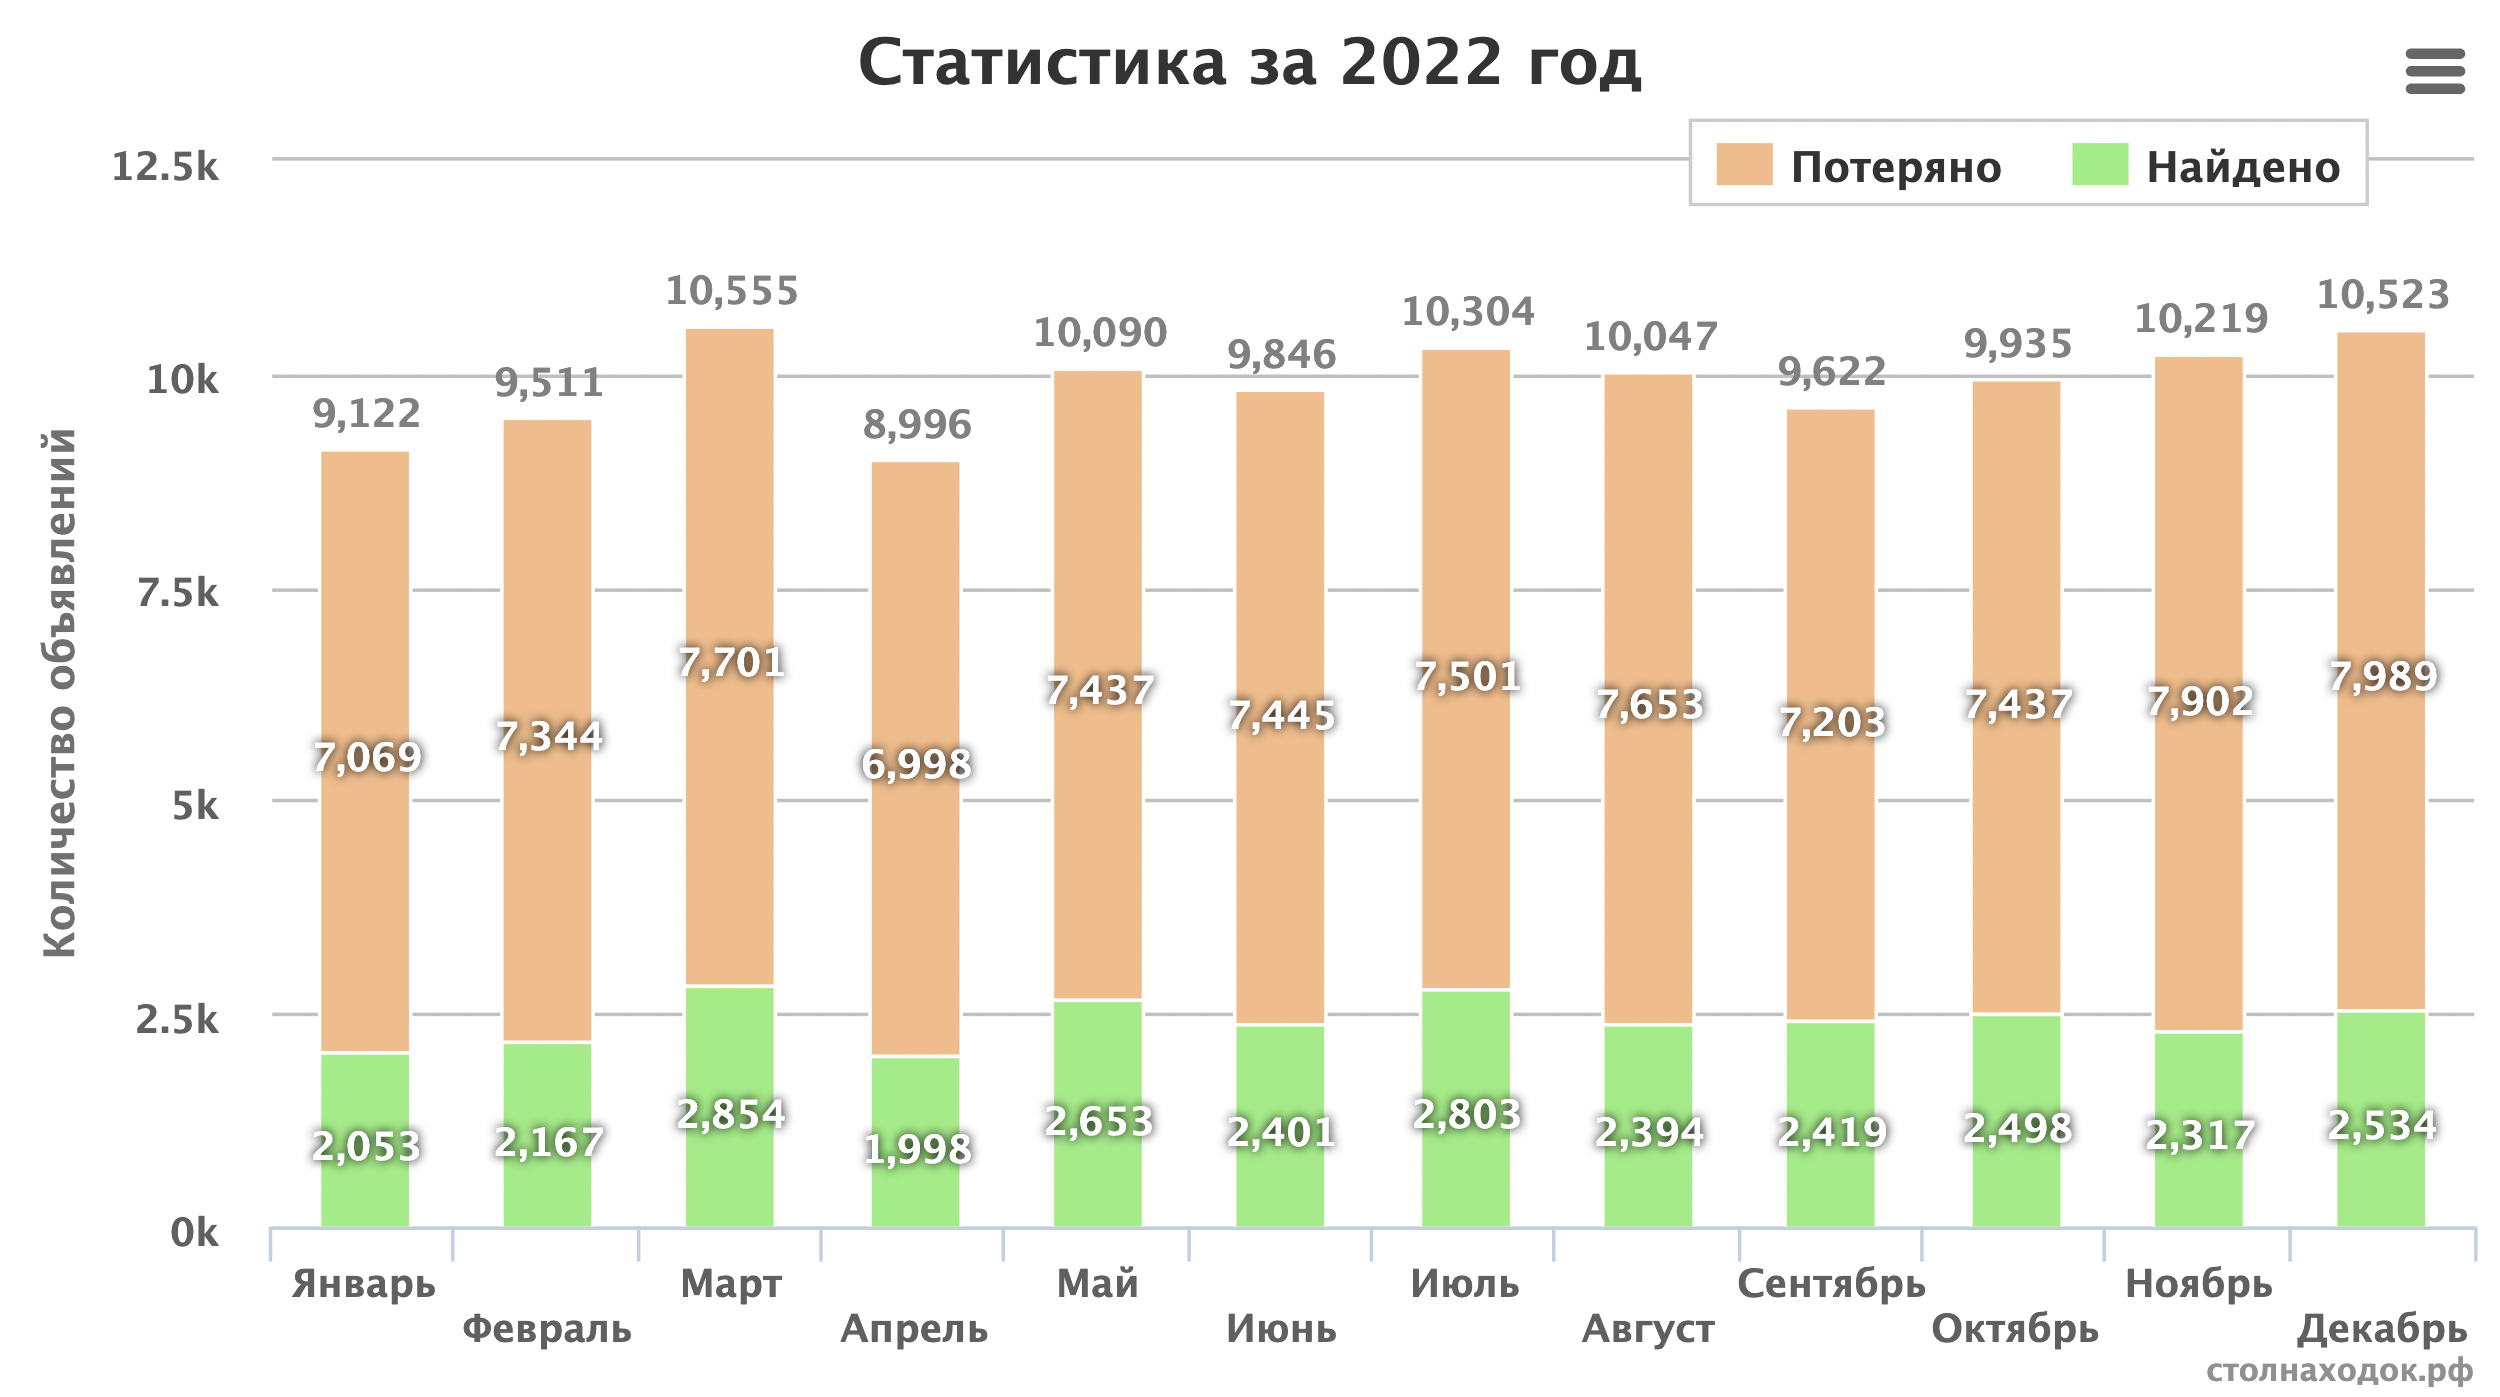
\includegraphics[width=.6\textwidth]{images/chart2022}
	\parskip=6pt
	\caption{Востребованность системы столнаходок.рф в 2022 году}
	\label{fig:chart2022}
\end{figure}

\subsection{Типы существующих решений для поиска и возврата утерянных вещей}

Существует несколько типов существующих решений для поиска и возврата утерянных вещей. Ниже приведены некоторые из них:
\begin{enumerate}
	\item Веб-сайты и приложения <<Бюро находок>>: Эти сервисы предоставляют платформу для регистрации утерянных вещей и поиска их владельцев. Пользователи могут создавать объявления о потерянных или найденных вещах и связываться друг с другом для возврата. Некоторые из этих сервисов предлагают возможность добавления фотографий или описания вещи для облегчения поиска.
	
	\item Технология RFID (Radio Frequency Identification): RFID-метки могут быть прикреплены к ценным вещам, и их сигнал может быть отслежен с помощью специального считывателя. Это позволяет пользователям быстро определить местоположение утерянных вещей через дополнительное программное обеспечение.
	
	\item GPS-трекеры: Эти устройства с GPS-модулем могут быть прикреплены к вещам, и их местоположение может быть отслежено с помощью специализированного приложения для смартфонов или веб-панели управления. Пользователи могут получать уведомления о перемещении вещи и быстро определить ее местонахождение.
	
	\item Автоматизированные системы обнаружения: Некоторые организации, такие как аэропорты или железнодорожные станции, имеют системы обнаружения утерянных вещей. Эти системы используют технологии, такие как видеонаблюдение, датчики движения или распознавание образов, чтобы отслеживать и возвращать потерянные вещи своим владельцам.
\end{enumerate}

Каждый из этих типов решений имеет свои преимущества и недостатки. Некоторые из них могут быть более подходящими для конкретных ситуаций, например, GPS-трекеры могут быть полезными при поиске утерянных вещей на открытой местности, в то время как RFID-метки могут быть более подходящими для использования внутри помещений. Веб-сайты и приложения <<Бюро находок>> предоставляют более универсальное решение, которое может быть использовано в различных ситуациях.

\subsection{Анализ существующих систем для поиска и возврата утерянных вещей}

В настоящем разделе будет проведен обзор существующих сервисов и приложений, которые предлагают функциональность поиска и возврата утерянных вещей. Данный обзор позволит выявить основные преимущества и недостатки этих сервисов, а также определить потенциальные возможности для улучшения их функциональности.

<<столнаходок.рф>>~\cite{bib:stol_nahodok} --- это один из наиболее популярных веб-сервисов, предоставляющих возможность объявлять о потерянных и найденных предметах. Сервис имеет простой и интуитивно понятный интерфейс, позволяющий пользователям быстро разместить информацию о потерянных вещах и связаться с владельцами найденных предметов. Однако, отсутствие системы уведомлений и неудобное сопоставление объявлений ограничивают его функциональность.

<<Find My Stuff>>~\cite{bib:find_my_stuff} --- это мобильное приложение, разработанное для операционных систем iOS и Android. Оно предлагает функцию отслеживания утерянных предметов через GPS-модуль смартфона. Пользователи могут отмечать свои вещи на карте и получать уведомления, когда они находятся рядом с утерянным предметом. Однако, ограничение использования только наличием смартфона с GPS-модулем и низкая точность определения местоположения представляют существенные ограничения данного приложения.

<<Lost Property Office>>~\cite{bib:parliament_lost_and_found} --- это веб-сервис, предоставляемый государственными организациями и органами правопорядка. Сервис позволяет пользователям сообщать о потерянных и найденных предметах, а также предоставляет информацию о процедуре возврата утерянных вещей. Однако, ограниченный доступ к сервису и неудобный процесс регистрации и подачи заявки являются значительными недостатками данного сервиса.

На основании проведенного обзора можно сделать вывод, что существующие веб-сервисы и приложения для поиска и возврата утерянных вещей имеют некоторые преимущества, но также недостатки, которые ограничивают их функциональность и удобство использования. Веб-сервис Бюро находок будет разработан с учетом этих недостатков и предлагать более удобное взаимодействие между пользователями и сервисом.

Ниже приведена сравнительная таблица~\ref{tab:analogs_comparison} основных характеристик и функций приведенных выше аналогов:
\begin{table}[htb]
	\caption{Сравнительная таблица аналогов}
	\centering
	
	\tolerance=0
	\emergencystretch=10pt
	\hyphenpenalty=0
	\exhyphenpenalty=0
	\begin{tabular}{ |p{2cm}|p{3cm}|p{2cm}|p{2cm}|p{3cm}|p{2cm}| } 
		\hline
		Сервис / Приложение & Интерфейс и удобство использования & Опове\-ще\-ния & Точность определения местоположения & Регистрация и подача заявки & Доступ\-ность \\ \hline
		
		стол\-на\-ходок.рф & Простой и интуитивно понятный интерфейс & Отсут\-ству\-ют & Не\-оп\-ре\-де\-ле\-но & Простой процесс регистрации & Широкий доступ \\ \hline
		
		Find My Stuff & Простой и интуитивно понятный интерфейс & Опо\-ве\-ще\-ния через уведомления & Низкая точность & Простой процесс регистрации & Доступен только на смартфонах с GPS \\ \hline
		
		Lost Property Office & Неудобный процесс регистрации и подачи заявки & Отсут\-ству\-ют & Не\-оп\-ре\-де\-ле\-но & Неудобный процесс регистрации и подачи заявки & Огра\-ни\-чен\-ный доступ \\ \hline
	\end{tabular}
	\label{tab:analogs_comparison}
\end{table}

\subsection*{Вывод по разделу}

В аналитическом разделе моего исследования проведен подробный обзор различных существующих веб-сервисов и приложений, которые предназначены для поиска и возврата утерянных вещей. Мы изучили и проанализировали их функциональность, особенности, преимущества и недостатки.

Веб-сервисы и приложения <<Бюро находок>> представляют собой одно из самых популярных и широко используемых решений в данной области. Они предоставляют платформу, на которой пользователи могут зарегистрировать утерянные вещи и связаться с их владельцами. Это позволяет упростить процесс поиска и возврата утерянных вещей, обеспечивая удобный и интуитивно понятный интерфейс для пользователей.\label{key}